% Options for packages loaded elsewhere
\PassOptionsToPackage{unicode}{hyperref}
\PassOptionsToPackage{hyphens}{url}
\PassOptionsToPackage{dvipsnames,svgnames,x11names}{xcolor}
%
\documentclass[
  xelatex,
  ja=standard]{bxjsarticle}

\usepackage{amsmath,amssymb}
\usepackage{iftex}
\ifPDFTeX
  \usepackage[T1]{fontenc}
  \usepackage[utf8]{inputenc}
  \usepackage{textcomp} % provide euro and other symbols
\else % if luatex or xetex
  \usepackage{unicode-math}
  \defaultfontfeatures{Scale=MatchLowercase}
  \defaultfontfeatures[\rmfamily]{Ligatures=TeX,Scale=1}
\fi
\usepackage{lmodern}
\ifPDFTeX\else  
    % xetex/luatex font selection
  \setmainfont[BoldFont=Noto Sans CJK JP]{Noto Serif CJK JP}
\fi
% Use upquote if available, for straight quotes in verbatim environments
\IfFileExists{upquote.sty}{\usepackage{upquote}}{}
\IfFileExists{microtype.sty}{% use microtype if available
  \usepackage[]{microtype}
  \UseMicrotypeSet[protrusion]{basicmath} % disable protrusion for tt fonts
}{}
\makeatletter
\@ifundefined{KOMAClassName}{% if non-KOMA class
  \IfFileExists{parskip.sty}{%
    \usepackage{parskip}
  }{% else
    \setlength{\parindent}{0pt}
    \setlength{\parskip}{6pt plus 2pt minus 1pt}}
}{% if KOMA class
  \KOMAoptions{parskip=half}}
\makeatother
\usepackage{xcolor}
\setlength{\emergencystretch}{3em} % prevent overfull lines
\setcounter{secnumdepth}{5}
% Make \paragraph and \subparagraph free-standing
\ifx\paragraph\undefined\else
  \let\oldparagraph\paragraph
  \renewcommand{\paragraph}[1]{\oldparagraph{#1}\mbox{}}
\fi
\ifx\subparagraph\undefined\else
  \let\oldsubparagraph\subparagraph
  \renewcommand{\subparagraph}[1]{\oldsubparagraph{#1}\mbox{}}
\fi


\providecommand{\tightlist}{%
  \setlength{\itemsep}{0pt}\setlength{\parskip}{0pt}}\usepackage{longtable,booktabs,array}
\usepackage{calc} % for calculating minipage widths
% Correct order of tables after \paragraph or \subparagraph
\usepackage{etoolbox}
\makeatletter
\patchcmd\longtable{\par}{\if@noskipsec\mbox{}\fi\par}{}{}
\makeatother
% Allow footnotes in longtable head/foot
\IfFileExists{footnotehyper.sty}{\usepackage{footnotehyper}}{\usepackage{footnote}}
\makesavenoteenv{longtable}
\usepackage{graphicx}
\makeatletter
\def\maxwidth{\ifdim\Gin@nat@width>\linewidth\linewidth\else\Gin@nat@width\fi}
\def\maxheight{\ifdim\Gin@nat@height>\textheight\textheight\else\Gin@nat@height\fi}
\makeatother
% Scale images if necessary, so that they will not overflow the page
% margins by default, and it is still possible to overwrite the defaults
% using explicit options in \includegraphics[width, height, ...]{}
\setkeys{Gin}{width=\maxwidth,height=\maxheight,keepaspectratio}
% Set default figure placement to htbp
\makeatletter
\def\fps@figure{htbp}
\makeatother

\renewcommand{\thefootnote}{\arabic{footnote}}
\makeatletter
\@ifpackageloaded{tcolorbox}{}{\usepackage[skins,breakable]{tcolorbox}}
\@ifpackageloaded{fontawesome5}{}{\usepackage{fontawesome5}}
\definecolor{quarto-callout-color}{HTML}{909090}
\definecolor{quarto-callout-note-color}{HTML}{0758E5}
\definecolor{quarto-callout-important-color}{HTML}{CC1914}
\definecolor{quarto-callout-warning-color}{HTML}{EB9113}
\definecolor{quarto-callout-tip-color}{HTML}{00A047}
\definecolor{quarto-callout-caution-color}{HTML}{FC5300}
\definecolor{quarto-callout-color-frame}{HTML}{acacac}
\definecolor{quarto-callout-note-color-frame}{HTML}{4582ec}
\definecolor{quarto-callout-important-color-frame}{HTML}{d9534f}
\definecolor{quarto-callout-warning-color-frame}{HTML}{f0ad4e}
\definecolor{quarto-callout-tip-color-frame}{HTML}{02b875}
\definecolor{quarto-callout-caution-color-frame}{HTML}{fd7e14}
\makeatother
\makeatletter
\makeatother
\makeatletter
\makeatother
\makeatletter
\@ifpackageloaded{caption}{}{\usepackage{caption}}
\AtBeginDocument{%
\ifdefined\contentsname
  \renewcommand*\contentsname{目次}
\else
  \newcommand\contentsname{目次}
\fi
\ifdefined\listfigurename
  \renewcommand*\listfigurename{図一覧}
\else
  \newcommand\listfigurename{図一覧}
\fi
\ifdefined\listtablename
  \renewcommand*\listtablename{表一覧}
\else
  \newcommand\listtablename{表一覧}
\fi
\ifdefined\figurename
  \renewcommand*\figurename{図}
\else
  \newcommand\figurename{図}
\fi
\ifdefined\tablename
  \renewcommand*\tablename{表}
\else
  \newcommand\tablename{表}
\fi
}
\@ifpackageloaded{float}{}{\usepackage{float}}
\floatstyle{ruled}
\@ifundefined{c@chapter}{\newfloat{codelisting}{h}{lop}}{\newfloat{codelisting}{h}{lop}[chapter]}
\floatname{codelisting}{コード}
\newcommand*\listoflistings{\listof{codelisting}{コード一覧}}
\makeatother
\makeatletter
\@ifpackageloaded{caption}{}{\usepackage{caption}}
\@ifpackageloaded{subcaption}{}{\usepackage{subcaption}}
\makeatother
\makeatletter
\@ifpackageloaded{tcolorbox}{}{\usepackage[skins,breakable]{tcolorbox}}
\makeatother
\makeatletter
\@ifundefined{shadecolor}{\definecolor{shadecolor}{rgb}{.97, .97, .97}}
\makeatother
\makeatletter
\makeatother
\makeatletter
\makeatother
\ifLuaTeX
\usepackage[bidi=basic]{babel}
\else
\usepackage[bidi=default]{babel}
\fi
\babelprovide[main,import]{japanese}
% get rid of language-specific shorthands (see #6817):
\let\LanguageShortHands\languageshorthands
\def\languageshorthands#1{}
\ifLuaTeX
  \usepackage{selnolig}  % disable illegal ligatures
\fi
\usepackage[]{natbib}
\bibliographystyle{jecon}
\IfFileExists{bookmark.sty}{\usepackage{bookmark}}{\usepackage{hyperref}}
\IfFileExists{xurl.sty}{\usepackage{xurl}}{} % add URL line breaks if available
\urlstyle{same} % disable monospaced font for URLs
\hypersetup{
  pdftitle={人工知能の機械学習},
  pdfauthor={土井翔平},
  pdflang={ja},
  colorlinks=true,
  linkcolor={NavyBlue},
  filecolor={Maroon},
  citecolor={NavyBlue},
  urlcolor={NavyBlue},
  pdfcreator={LaTeX via pandoc}}

\title{人工知能の機械学習}
\usepackage{etoolbox}
\makeatletter
\providecommand{\subtitle}[1]{% add subtitle to \maketitle
  \apptocmd{\@title}{\par {\large #1 \par}}{}{}
}
\makeatother
\subtitle{技術政策学(データ科学編)}
\author{土井翔平}
\date{2023-05-22}

\begin{document}
\maketitle
\ifdefined\Shaded\renewenvironment{Shaded}{\begin{tcolorbox}[interior hidden, sharp corners, borderline west={3pt}{0pt}{shadecolor}, boxrule=0pt, enhanced, frame hidden, breakable]}{\end{tcolorbox}}\fi

\hypertarget{ux306fux3058ux3081ux306b}{%
\section*{はじめに}\label{ux306fux3058ux3081ux306b}}
\addcontentsline{toc}{section}{はじめに}

\begin{tcolorbox}[enhanced jigsaw, opacitybacktitle=0.6, colbacktitle=quarto-callout-warning-color!10!white, leftrule=.75mm, titlerule=0mm, arc=.35mm, left=2mm, coltitle=black, breakable, colframe=quarto-callout-warning-color-frame, bottomtitle=1mm, toptitle=1mm, toprule=.15mm, colback=white, rightrule=.15mm, title=\textcolor{quarto-callout-warning-color}{\faExclamationTriangle}\hspace{0.5em}{警告}, bottomrule=.15mm, opacityback=0]

日進月歩の分野なので、本章の内容はすぐに古いものになる(or既にそうであるかもしれない)点に注意。

\end{tcolorbox}

ビッグデータは魅力的な資源(材料)だが、有効な利用法(調理法)があって初めて価値を持つ。

\(\leadsto\)近年のデータ科学における2つの変革

\begin{enumerate}
\def\labelenumi{\arabic{enumi}.}
\tightlist
\item
  機械学習:データから一定のパターンを機械(パソコン)が学習し、\textbf{予測をする}。
\item
  因果推論:データから因果関係(因果効果)を学習する。
\end{enumerate}

\(\leadsto\)いわゆる(最近において)人工知能と呼ばれるものは機械学習(予測)

\begin{itemize}
\tightlist
\item
  現在は第3次人工知能ブームと言われている。
\item
  クオリティが高いがゆえに、あたかも機械が人間のように思考しているように見えてしまう。
\item
  自然言語処理に関するタスク\href{https://super.gluebenchmark.com/}{SuperGLUE}では人間を越えている。
\end{itemize}

\textbf{生成 (generative) AI}:ある情報から、別の情報を出力するモデル

\begin{itemize}
\tightlist
\item
  \textbf{大規模言語モデル} (large language model:
  LLM):大量のテキストを使い、巨大なモデルを学習した生成AI

  \begin{itemize}
  \tightlist
  \item
    \href{https://openai.com/blog/chatgpt}{ChatGPT}、\href{https://bard.google.com/}{Google
    Bard}、\href{https://www.microsoft.com/ja-jp/bing}{Microsoft Bing
    AI}など
  \item
    GPT=\textbf{Generative} Pre-trained Trensformer
  \item
    まずは、\href{https://platform.openai.com/examples}{OpenAIのPlayground}で遊んでみよう。
  \end{itemize}
\item
  画像生成の性能も向上、Vision and Languageの発展

  \begin{itemize}
  \tightlist
  \item
    \href{https://openai.com/dall-e-2/}{DALL·E 2}
    、\href{https://www.midjourney.com/}{midjourney}
    、\href{https://huggingface.co/spaces/stabilityai/stable-diffusion}{stable
    difffusion} など
  \end{itemize}
\end{itemize}

生成モデルも実は予測の組み合わせである。

\begin{itemize}
\tightlist
\item
  \href{https://www.deepl.com/translator}{DeepL}\(\leadsto\)ある言語の文章から他の言語の文章を予測する。
\item
  チャットbot、文書要約、コード生成\(\leadsto\)ある文章から返答、要約、次に来る文章を予測する。
\item
  AmazonやNetflixの推薦\(\leadsto\)これまでの購入履歴やウォッチリストから次に購入する商品を予測する。
\item
  学習過程にテキストデータを含めることで、テキストから画像生成できる
  (vision and language) 。
\end{itemize}

代表的な機械学習の分類

\begin{enumerate}
\def\labelenumi{\arabic{enumi}.}
\tightlist
\item
  \textbf{教師あり学習}:特徴量 (feature) から対象を予測する。
\item
  \textbf{教師なし学習}:多様な特徴量から重要なものを抽出する。
\item
  \textbf{強化学習}:フィードバックを通じて最適な方策 (policy)
  を発見する。
\end{enumerate}

\(\leadsto\)これらの概要を理解し、生成AIが何をしているかを理解する。

\hypertarget{ux6559ux5e2bux3042ux308aux5b66ux7fd2}{%
\section{教師あり学習}\label{ux6559ux5e2bux3042ux308aux5b66ux7fd2}}

教師あり学習とは、機械に人間の判断のパターンを学習させ、模倣できるようにすること。

\(\leadsto\)言い換えれば、\textbf{予測} (prediction)
というタスクを実行できるように訓練する。

\begin{itemize}
\tightlist
\item
  写真とその内容のペアのデータを機械に覚えさせる。
\item
  住宅の情報(間取り、最寄り駅までの距離\ldots\ldots etc)と価格を機械に覚えさせる。
\end{itemize}

\begin{figure}[htpb]

{\centering \includegraphics{machine_learning_files/mediabag/l_bit202012111543429.jpg}

}

\caption{\href{https://www.sbbit.jp/article/cont1/49067}{教師あり学習のイメージ}}

\end{figure}

\(\leadsto\)ある情報を入力すると、それに対応する情報を出力する。

\begin{itemize}
\tightlist
\item
  入力情報に対応する出力(正解)を人間が判断する\textbf{アノテーション}が重要になる。
\end{itemize}

\hypertarget{ux56deux5e30ux5206ux6790}{%
\subsection{回帰分析}\label{ux56deux5e30ux5206ux6790}}

シンプルで、広く使われている教師あり学習の手法として\textbf{回帰分析}
(regression analysis) がある。

\begin{itemize}
\tightlist
\item
  例えば、北海道の中古マンション価格の教師あり学習を行ってみる。
\end{itemize}

\begin{figure}[htpb]

{\centering 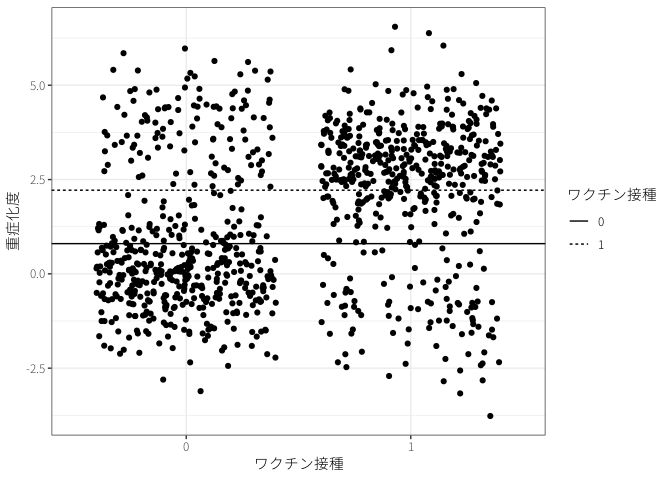
\includegraphics{machine_learning_files/figure-pdf/unnamed-chunk-2-1.png}

}

\end{figure}

\[
\textrm{価格} = 335.58 + 11.84 \times \textrm{広さ}
\]

\textbf{最小二乗法} (ordinary least squares: OLS)
はデータとの誤差が最も小さくなる直線を計算する。

\begin{itemize}
\tightlist
\item
  予測値を一次関数(直線)で予測する。
\end{itemize}

\[
i\textrm{の予測値} = \hat{y}_i = \underbrace{\hat{\alpha}}_{\textrm{切片 (intercept)}} 
+ \underbrace{\hat{\beta}}_{\textrm{傾き (slope)}} x_i
\]

\begin{itemize}
\tightlist
\item
  \(i\)は個体ごとに異なる値を取るということを意味している。
\item
  上手く予測できるような\(\hat{\alpha}, \hat{\beta}\)をデータから求める(学習する)。
\item
  真の値と予測値のズレ、誤差 (error) が小さい方がいいはず。
\end{itemize}

\[
i\textrm{の予測誤差} = i\textrm{の真の値} - i\textrm{の予測値} = y_i - \hat{y}_i
\]

\begin{itemize}
\tightlist
\item
  ズレはプラスにもマイナスにもなるので、プラスの値しか取らない距離や面積に変換する。
\item
  通常は誤差を二乗して、面積にする。
\end{itemize}

\[
i\textrm{の予測誤差の二乗} = i\textrm{の真の値} - i\textrm{の予測値} = (y_i - \hat{y}_i)^2
\]

\begin{itemize}
\tightlist
\item
  個々の誤差をデータ全体について計算し、合計する。
\end{itemize}

\[
i\textrm{の予測誤差の二乗の合計} = (y_1 - \hat{y}_1)^2 + (y_2 - \hat{y}_2)^2 + \cdots
\]

\(\leadsto\)これを最小にする\(\hat{\alpha}, \hat{\beta}\)をデータから求める!(パソコンが計算してくれる)\footnote{最適化(偏微分係数が0となる値を求める)によって明示的に解くことができる。}

\begin{itemize}
\tightlist
\item
  \(\hat{\alpha}, \hat{\beta}\)は\(\hat{y}_i\)の中に入っていることに注意。
\end{itemize}

予測に使う情報(特徴量)は1つである必要はない。

\[
\textrm{価格} = 396.27 + 12.50 \times \textrm{広さ} -10.57 \times \textrm{距離}
\]

\begin{itemize}
\tightlist
\item
  パターンを学習しているだけであり、機械がマンションについて理解しているわけではない。
\end{itemize}

予測対象がカテゴリーの場合はどうするのか?

\begin{itemize}
\tightlist
\item
  機械学習の代表的なデータセットに\href{https://www.kaggle.com/competitions/titanic}{タイタニック号の乗客データ}がある。
\item
  このときの予測対象は乗客が生存したかどうかというカテゴリー
\end{itemize}

\(\leadsto\)\textbf{ロジスティック関数}(シグモイド関数)を使って変形すると、0から1の間に収まる。

\begin{figure}[htpb]

{\centering 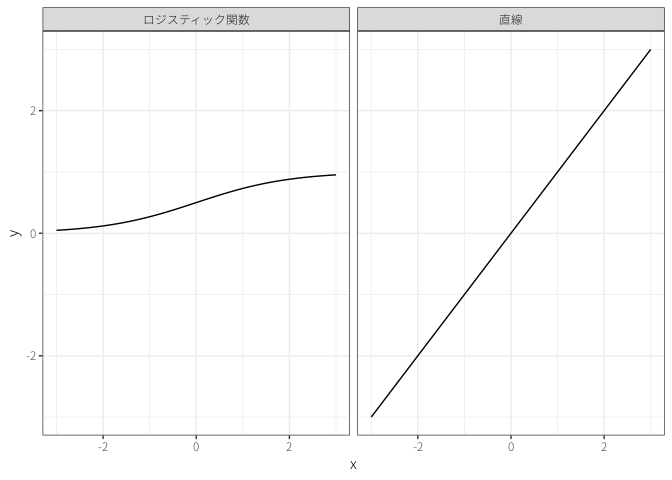
\includegraphics{machine_learning_files/figure-pdf/unnamed-chunk-3-1.png}

}

\end{figure}

\hypertarget{ux6c7aux5b9aux6728}{%
\subsection{決定木}\label{ux6c7aux5b9aux6728}}

回帰分析以外の代表的な教師あり学習の手法として\textbf{決定木} (decision
tree) がある。

\begin{figure}[htpb]

{\centering \includegraphics{machine_learning_files/mediabag/image001.png}

}

\caption{\href{https://www.nttcoms.com/service/research/dataanalysis/decision-tree/}{決定木のイメージ}}

\end{figure}

\(\leadsto\)弱い決定木をたくさん集めた\textbf{ランダム・フォレスト}(やその発展形\footnote{XGBoostやLightGBMなど。})がよく使われている。

\begin{itemize}
\tightlist
\item
  三人寄れば文殊の知恵? 陪審定理?
\end{itemize}

\hypertarget{ux6df1ux5c64ux5b66ux7fd2}{%
\subsection{深層学習}\label{ux6df1ux5c64ux5b66ux7fd2}}

深層学習 (deep learning) は深層ニューラル・ネットワーク (deep neural
network: DNN) とも呼ばれる。

\(\leadsto\)もともとは人間のニューロンをマシン上で再現すれば人工知能ができるかもという期待

\begin{itemize}
\tightlist
\item
  閾値を超えると発火して信号を送信する。
\end{itemize}

\begin{figure}[htpb]

{\centering 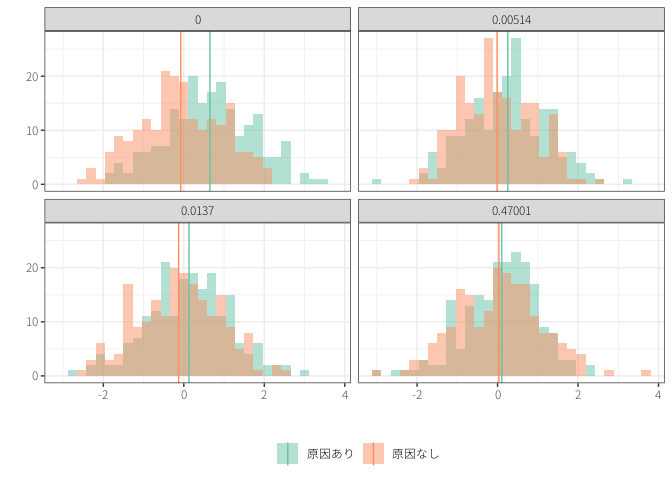
\includegraphics{machine_learning_files/figure-pdf/unnamed-chunk-4-1.png}

}

\end{figure}

\(\leadsto\)回帰分析をニューロンとして見て\footnote{厳密に言えば、活性化関数を挟む。}、これをたくさん作る。

\begin{figure}[htpb]

{\centering 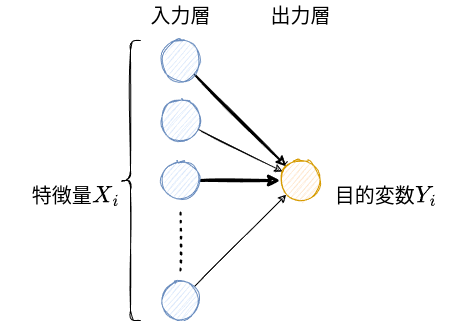
\includegraphics{figures/logistic_regression.drawio.png}

}

\caption{ロジスティック回帰のイメージ}

\end{figure}

\begin{figure}[htpb]

{\centering 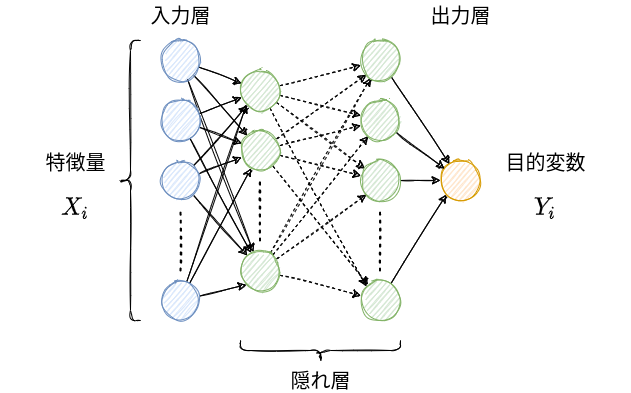
\includegraphics{figures/deep_learning.drawio.png}

}

\caption{深層ニューラル・ネットワークのイメージ}

\end{figure}

なぜ深層学習はすごいのか?

\begin{enumerate}
\def\labelenumi{\arabic{enumi}.}
\tightlist
\item
  隠れ層を増やせば増やすほど柔軟な予測ができる。

  \begin{itemize}
  \tightlist
  \item
    パラメータの数(隠れ層の数に比例)\(\approx\)モデルのサイズ
  \item
    例えば\[\hat{y}_i = \hat{\alpha} + \hat{\beta} x_i\]のパラメータの数は2
  \end{itemize}
\item
  特徴量を人間が作らなくてよい。

  \begin{itemize}
  \tightlist
  \item
    むしろ、重要な特徴量がなにかを学習する(\textbf{表現学習})。
  \end{itemize}
\item
  学習済みモデルを使える。

  \begin{itemize}
  \tightlist
  \item
    タスクに応じて出力側を再学習(\textbf{ファイン・チューニング})する。
  \item
    GPT=Generative \textbf{Pre-trained} Trensformer
  \end{itemize}
\item
  様々な形式のデータ(テキスト、画像、音声\ldots\ldots)を同じ枠組みで分析できる。

  \begin{itemize}
  \tightlist
  \item
    vision and languageなど\textbf{マルチモーダル}なモデルの開発
  \end{itemize}
\end{enumerate}

\(\leadsto\)生成AI(LLM含む)は与えられた単語の列から、次に来そうな、もっともらしい単語を予測している(だけ)!

\begin{figure}[htpb]

{\centering 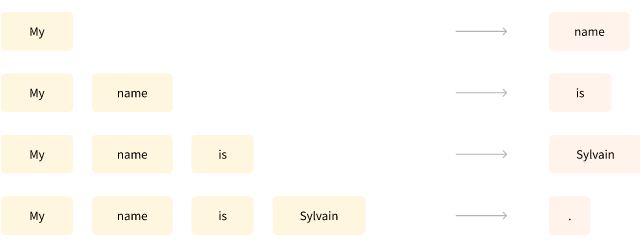
\includegraphics{figures/causal_modeling.png}

}

\caption{\href{https://huggingface.co/learn/nlp-course/ja/chapter1/4}{LLMによる文書生成のイメージ}}

\end{figure}

\begin{itemize}
\tightlist
\item
  同じ入力に対して同じ回答をしないように、ある程度ランダムに予測をしている。

  \begin{itemize}
  \tightlist
  \item
    GPTにおけるtemparatureはランダム度合いを指定している。
  \end{itemize}
\item
  人工知能の獲得か?(例、中国語の部屋)
\end{itemize}

\hypertarget{ux30d7ux30edux30f3ux30d7ux30c8ux30a8ux30f3ux30b8ux30cbux30a2ux30eaux30f3ux30b0}{%
\subsection{プロンプト・エンジニアリング}\label{ux30d7ux30edux30f3ux30d7ux30c8ux30a8ux30f3ux30b8ux30cbux30a2ux30eaux30f3ux30b0}}

ChatGPTなどの最近のLLMがすごいのは、タスクも指示するだけでよいこと。

\begin{itemize}
\tightlist
\item
  翻訳、要約、質疑応答などのタスクごとにモデルを作らなくて良い。
\end{itemize}

\(\leadsto\)入力する指示文(\textbf{プロンプト})をどのようにするのかが重要。

\begin{itemize}
\tightlist
\item
  プロンプトの書き方を工夫することをプロンプト・エンジニアリングなどと呼ぶ。
\item
  いくつかの具体例を提示すると、性能が良くなる、安定する\textbf{few shot
  learning}という現象(?)
\end{itemize}

\hypertarget{ux62e1ux6563ux30e2ux30c7ux30eb}{%
\subsection{拡散モデル}\label{ux62e1ux6563ux30e2ux30c7ux30eb}}

拡散モデル:画像にノイズを追加していって、それを取り除くプロセスを学習

\begin{figure}[htpb]

{\centering \includegraphics{machine_learning_files/mediabag/06_m.png}

}

\caption{\href{https://gigazine.net/news/20221006-visuals-explaining-stable-diffusion/}{拡散モデルのイメージ}}

\end{figure}

\begin{figure}[htpb]

{\centering \includegraphics{machine_learning_files/mediabag/08_m.png}

}

\caption{\href{https://gigazine.net/news/20221006-visuals-explaining-stable-diffusion/}{拡散モデルのイメージ}}

\end{figure}

\(\leadsto\)テキストからの画像生成もテキスト→画像の予測を行っている。

\hypertarget{ux6559ux5e2bux306aux3057ux5b66ux7fd2}{%
\section{教師なし学習}\label{ux6559ux5e2bux306aux3057ux5b66ux7fd2}}

数値ではない文書データをどのようにデータ分析するのか?

\begin{itemize}
\tightlist
\item
  シンプルな方法は\textbf{bag of
  words}(単語の出現頻度を特徴量とする)アプローチ
\end{itemize}

\(\leadsto\)教師なし学習によってデータから特徴量を抽出する。

\hypertarget{ux5358ux8a9eux57cbux3081ux8fbcux307f}{%
\subsection{単語埋め込み}\label{ux5358ux8a9eux57cbux3081ux8fbcux307f}}

\textbf{単語埋め込み} (word
embedding):単語を低次元空間のベクトルに変換する

\(\leadsto\)単語のベクトル(位置)\(\approx\)意味?

\begin{figure}[htpb]

{\centering 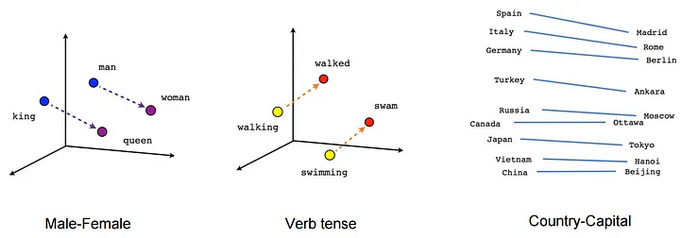
\includegraphics{figures/word_embeddings.png}

}

\caption{\href{https://towardsdatascience.com/creating-word-embeddings-coding-the-word2vec-algorithm-in-python-using-deep-learning-b337d0ba17a8}{単語埋め込みのイメージ}}

\end{figure}

\begin{itemize}
\tightlist
\item
  単語の意味は周辺の単語によって決まるはず。
\end{itemize}

\begin{figure}[htpb]

{\centering 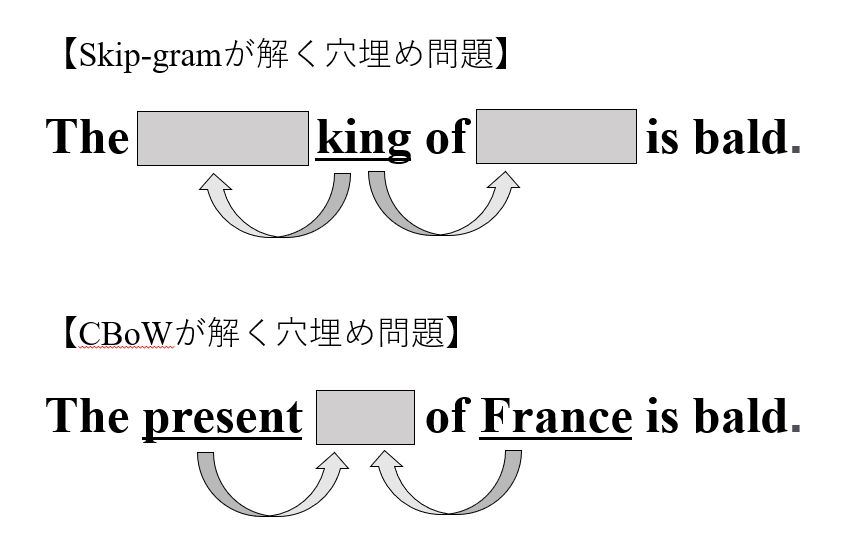
\includegraphics{figures/word_embeddings2.png}

}

\caption{\href{https://ainow.ai/2021/04/08/254071/}{単語埋め込みの学習のイメージ}}

\end{figure}

\(\leadsto\)周辺の単語をうまく予測できるベクトルを学習する。

\begin{itemize}
\tightlist
\item
  画像も同様に埋め込むことで、テキスト→画像の予測が可能となる。
\end{itemize}

\hypertarget{ux81eaux5df1ux6ce8ux610fux6a5fux69cb}{%
\subsection{自己注意機構}\label{ux81eaux5df1ux6ce8ux610fux6a5fux69cb}}

近年の自然言語処理の飛躍的発展のキーは\textbf{Transformer}\citep{vaswani2017}の登場\footnote{Transformerを提案したのはGoogleの研究者たち。}

\begin{itemize}
\tightlist
\item
  BERT=Bidirectional Encoder Representations from \textbf{Transformers}
\item
  GPT=Generative Pre-trained \textbf{Trensformer}
\end{itemize}

\begin{figure}[htpb]

{\centering 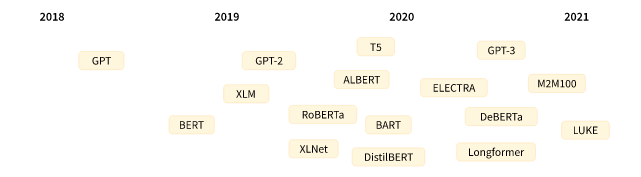
\includegraphics{figures/transformers.png}

}

\caption{\href{https://huggingface.co/learn/nlp-course/ja/chapter1/4?}{TransformerベースのLLM}}

\end{figure}

\(\leadsto\)特に\textbf{自己注意機構} (self-attention mechanism)
が重要(と言われている)

\begin{itemize}
\tightlist
\item
  ある単語を処理する際に、他のどの単語に注目すればよいのかを学習する。
\item
  ``Attention is all you need''\citep{vaswani2017}
\end{itemize}

\begin{figure}[htpb]

{\centering \includegraphics{machine_learning_files/mediabag/transformer_self-att.png}

}

\caption{\href{https://jalammar.github.io/illustrated-transformer/}{自己注意機構のイメージ}}

\end{figure}

\begin{itemize}
\tightlist
\item
  離れた単語も踏まえた学習ができる。
\item
  学習速度が高速になる。\footnote{並列化が可能になるため。}
\end{itemize}

\hypertarget{ux5f37ux5316ux5b66ux7fd2}{%
\section{強化学習}\label{ux5f37ux5316ux5b66ux7fd2}}

一部のモデルでは強化学習を用いて、更に性能を向上させている。

\begin{itemize}
\tightlist
\item
  例、GPT-3やそれ以上のベースと考えられているInstructGPT
\end{itemize}

強化学習では機械が最適なアクションを見つける。

\begin{itemize}
\tightlist
\item
  データからパターンを発見するわけではない。
\item
  エージェントが状態→行動→環境→報酬・状態を繰り返し、報酬を大きくする行動を発見する。
\end{itemize}

\begin{figure}[htpb]

{\centering \includegraphics{machine_learning_files/mediabag/1024px-Reinforcement.png}

}

\caption{\href{https://commons.wikimedia.org/wiki/File:Reinforcement_learning_diagram.svg}{強化学習のイメージ}}

\end{figure}

\hypertarget{alphago}{%
\subsection{AlphaGo}\label{alphago}}

AlphaGoは強化学習で囲碁のアルゴリズムを学習し2016年に世界トップ棋士に勝利

\begin{itemize}
\tightlist
\item
  初期設定として実際の棋譜データから学習したアルゴリズムを使用
\item
  2つのエージェント(機械)が対戦する中で大量にデータを生成し、学習
\end{itemize}

\begin{figure}[htpb]

{\centering \includegraphics{machine_learning_files/mediabag/41586_2016_BFnature1.jpg}

}

\caption{\citet{silver2016}}

\end{figure}

\hypertarget{ux4ebaux9593ux306eux30d5ux30a3ux30fcux30c9ux30d0ux30c3ux30af}{%
\subsection{人間のフィードバック}\label{ux4ebaux9593ux306eux30d5ux30a3ux30fcux30c9ux30d0ux30c3ux30af}}

InstructGPTでは人間のフィードバックからの強化学習 (Reinforcement
Learning from Human Feedback: RLHF) を用いている。

\begin{enumerate}
\def\labelenumi{\arabic{enumi}.}
\tightlist
\item
  プロンプトと(人間の作った)回答のデータから教師あり学習
\item
  1で作ったモデルの回答結果と人間の採点結果のデータから教師あり学習
\item
  1と2のモデルを使ってプロンプト→回答→採点の強化学習
\end{enumerate}

\begin{figure}[htpb]

{\centering 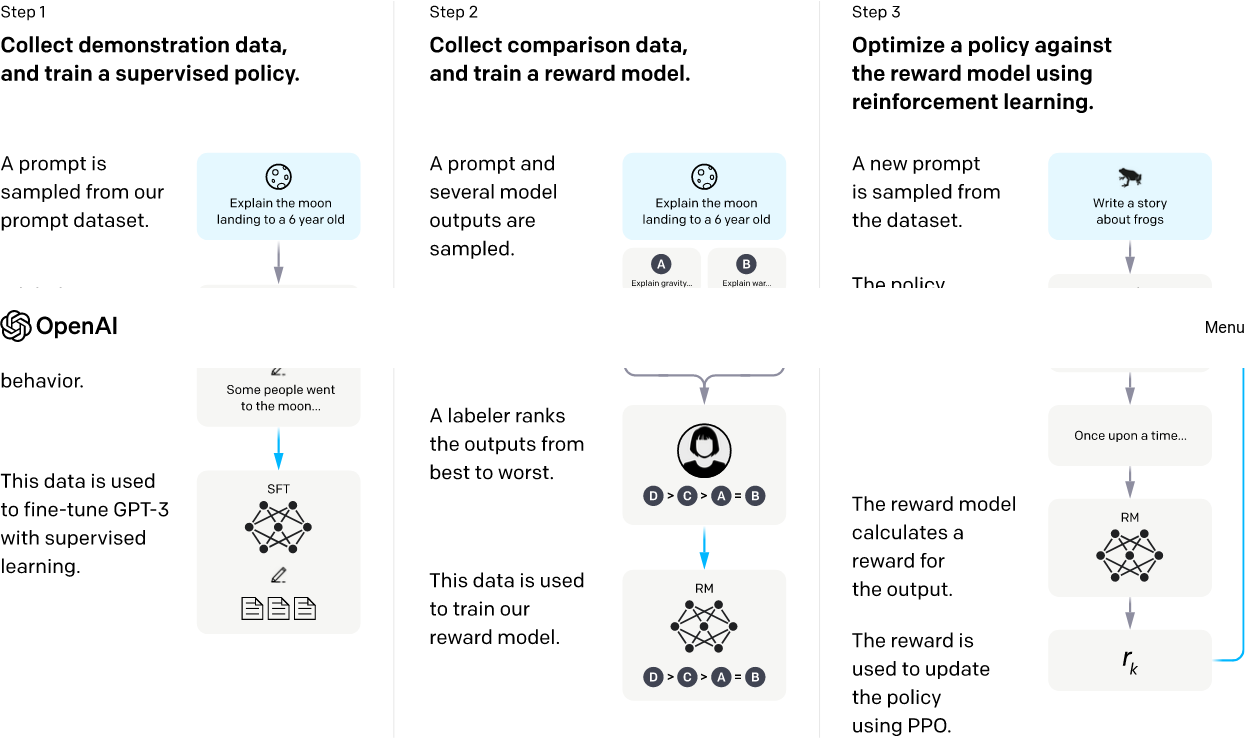
\includegraphics{figures/instructGPT.png}

}

\caption{\href{https://openai.com/research/instruction-following}{Aligning
language models to follow instructions}}

\end{figure}

\hypertarget{ux4ebaux5de5ux77e5ux80fdux306eux793eux4f1aux7684ux8ab2ux984c}{%
\section{人工知能の社会的課題}\label{ux4ebaux5de5ux77e5ux80fdux306eux793eux4f1aux7684ux8ab2ux984c}}

あらゆる技術がそうであるように、新しい技術の登場、急速な普及は様々な問題を引き起こしうる。

\begin{itemize}
\tightlist
\item
  G7広島サミットで生成AIに関するルールを策定する広島AIプロセスの立ち上げに合意
\end{itemize}

\hypertarget{ux4ebaux5de5ux77e5ux80fdux306eux4f7fux3044ux65b9}{%
\subsection{人工知能の使い方}\label{ux4ebaux5de5ux77e5ux80fdux306eux4f7fux3044ux65b9}}

\hypertarget{ux4ebaux5de5ux77e5ux80fdux306eux60aaux7528}{%
\subsubsection{人工知能の悪用}\label{ux4ebaux5de5ux77e5ux80fdux306eux60aaux7528}}

AIを悪用\(\leadsto\)偽の情報を作り、拡散

\begin{itemize}
\tightlist
\item
  文書生成 \(\leadsto\)
  \href{https://www.itmedia.co.jp/business/articles/2007/29/news025_4.html}{フェイクニュース}
\item
  物体検出 \& 画像生成 \(\leadsto\)
  \href{https://wired.jp/2018/09/14/deepfake-fake-videos-ai/}{Deep Fake}
\end{itemize}

\(\leadsto\)Deep
Fakeはオンラインの画像や映像を加工\(\leadsto\)フェイクポルノなど深刻な被害の可能性

\begin{figure}[htpb]

{\centering \includegraphics[width=0.5\textwidth,height=\textheight]{machine_learning_files/mediabag/20210504ax05S_o.jpg}

}

\caption{Deep Fakeの例}

\end{figure}

\begin{itemize}
\tightlist
\item
  ちなみに、スクリーンショットの捏造は人工知能を使わなくても簡単にできる。
\end{itemize}

どんな技術も悪用しようと思えばできる\(\leadsto\)(個人的に)重要なのは、悪用よりも誤用

\hypertarget{ux4ebaux5de5ux77e5ux80fdux306eux8aa4ux7528}{%
\subsubsection{人工知能の誤用}\label{ux4ebaux5de5ux77e5ux80fdux306eux8aa4ux7528}}

\textbf{統計的差別} (statistical discrimination)
:個人の属性(属する集団)に基づく差別

\begin{itemize}
\tightlist
\item
  学歴、性別、人種などで就職活動、賃貸契約、判決が異なる。
\end{itemize}

\(\leadsto\)機械学習はあくまで「人間を模倣」するので、人間に(無意識でも)差別があれば、\href{https://ainow.ai/2020/02/17/183256/}{機械はそれを学習}する。

アメリカの一部の州では保釈や刑期を決定する際にCOMPASというシステムでリスク評価を行っていた。

\begin{itemize}
\tightlist
\item
  黒人では「再犯する」と予測されたが「再犯しなかった」という間違いが多かった。
\item
  白人では「再犯しない」と予測されたが「再犯した」という間違いが多かった。
\end{itemize}

\begin{figure}[htpb]

{\centering \includegraphics{machine_learning_files/mediabag/F1.large.jpg}

}

\caption{\href{https://www.axion.zone/is-the-recidivism-prediction-algorithm-fair-to-race/}{COMPASSによる再犯予測}}

\end{figure}

学習に用いるデータが偏っている\(\leadsto\)予測も偏る。

\begin{figure}[htpb]

{\centering \includegraphics{machine_learning_files/mediabag/00_m.jpg}

}

\caption{\href{https://gigazine.net/news/20200702-twitter-ai-machine-learning-racism/}{偏ったデータによる学習}}

\end{figure}

\(\leadsto\)公平性のある機械学習を行う必要がある。

\textbf{敵対的攻撃} (adversarial attack) :あえてAIを騙すような情報入力

\begin{figure}[htpb]

{\centering \includegraphics{machine_learning_files/mediabag/00_m1.jpg}

}

\caption{\href{https://gigazine.net/news/20211130-universal-naturalistic-adversarial-patches/}{敵対的攻撃}}

\end{figure}

ChatGPTなどで指摘されているのは\textbf{幻覚} (hallucination)
と呼ばれる現象

\begin{itemize}
\tightlist
\item
  正しくない回答をあたかも正しいものと堂々と提示する。
\end{itemize}

意図せざる形での著作権侵害や個人情報流出も?

\begin{itemize}
\tightlist
\item
  学習に使用されたデータがほとんどそのまま出力される可能性
\end{itemize}

\(\leadsto\)AIだからといって客観的であるわけでも、常識的であるわけでもない。

\begin{itemize}
\tightlist
\item
  特に深層学習の中身はブラックボックスであり、\textbf{説明可能性}に欠けている。
\item
  回帰分析や決定木は分かりやすい。
\end{itemize}

\hypertarget{ux4ebaux5de5ux77e5ux80fdux3068ux502bux7406}{%
\subsubsection{人工知能と倫理}\label{ux4ebaux5de5ux77e5ux80fdux3068ux502bux7406}}

AI倫理、公平性のあるAIなどが必要

\(\leadsto\)AIが守るべき倫理、公平性とは?

自動運転車がトロッコ問題に遭遇したとき、どうすべきなのか?

\href{https://www.moralmachine.net/hl/ja}{モラル・マシン}というアンケートに答えることで、どのような命を重視するのかが分かる。

\begin{itemize}
\tightlist
\item
  「審査を始める」を押す。
\item
  直進する場合は左の絵を、曲がる場合は右の絵をクリックする。

  \begin{itemize}
  \tightlist
  \item
    ドクロマークがついている人が死んでしまうとする。
  \end{itemize}
\end{itemize}

\begin{figure}[htpb]

{\centering \includegraphics{machine_learning_files/mediabag/41586_2018_637_Fig2_.png}

}

\caption{\citet{awad2018}}

\end{figure}

倫理観は国ごとに異なる。

\begin{figure}[htpb]

{\centering \includegraphics{machine_learning_files/mediabag/d41586-018-07135-0_1.png}

}

\caption{\href{https://www.nature.com/articles/d41586-018-07135-0}{AI倫理観の地域ごとの違い}}

\end{figure}

\href{https://www.technologyreview.com/2018/10/24/139313/a-global-ethics-study-aims-to-help-ai-solve-the-self-driving-trolley-problem/}{日本の場合は}、

\begin{enumerate}
\def\labelenumi{\arabic{enumi}.}
\tightlist
\item
  お年寄りを助け、
\item
  より多くの人を助けるわけではなく、
\item
  歩行者を助ける
\end{enumerate}

傾向にあるらしい。

\begin{enumerate}
\def\labelenumi{\arabic{enumi}.}
\tightlist
\item
  人工知能は人間に代わって倫理的判断を行うわけではない。

  \begin{itemize}
  \tightlist
  \item
    人工知能に期待する倫理も人々、国々の間で同じではない。
  \end{itemize}
\item
  人工知能は誤作動も起こりうる。
\end{enumerate}

\(\leadsto\)人工知能の責任はどこにあるのか?

\begin{itemize}
\tightlist
\item
  \href{https://elsi.osaka-u.ac.jp/research/2120}{生成AI(Generative
  AI)の倫理的・法的・社会的課題(ELSI)論点の概観:2023年3月版(大阪大学)}
\end{itemize}

\hypertarget{ux4ebaux5de5ux77e5ux80fdux3068ux5175ux5668}{%
\subsubsection{人工知能と兵器}\label{ux4ebaux5de5ux77e5ux80fdux3068ux5175ux5668}}

無人兵器とAI技術の発展は\href{https://www.mofa.go.jp/mofaj/dns/ca/page24_001191.html}{自律型致死兵器システム}
(Lethal Autonomous Weapons Systems: LAWS)
の可能性を現実のものとしつつある。

\begin{itemize}
\tightlist
\item
  人間の代わりに戦闘をさせることで人命の損失を減らせる/戦争やテロリズムが起こりやすくなる?
\item
  人道法の違反(文民の殺害など)を起こす?

  \begin{itemize}
  \tightlist
  \item
    誤作動だけでなく、現在のAI技術ではAIの判断を人間が理解できない可能性
  \end{itemize}
\end{itemize}

\(\leadsto\)\href{https://jsil.jp/archives/expert/2020-10}{LAWS規制に関する議論の指針}が2019年に定まったばかり。

\hypertarget{ux4ebaux5de5ux77e5ux80fdux3068ux793eux4f1a}{%
\subsection{人工知能と社会}\label{ux4ebaux5de5ux77e5ux80fdux3068ux793eux4f1a}}

\hypertarget{ux4ebaux5de5ux77e5ux80fdux3068ux653fux6cbb}{%
\subsubsection{人工知能と政治}\label{ux4ebaux5de5ux77e5ux80fdux3068ux653fux6cbb}}

AIと民主主義の関わりに着目されつつある?

\begin{itemize}
\tightlist
\item
  AIが人間に代わって政策を決定する。
\item
  AIが個人の思考を学習して人間の代わりに政治(議論や投票\ldots\ldots)をする。
\item
  AIが議論や情報収集をアシストする。
\end{itemize}

科学技術を巡って展開される政治がある。

\(\leadsto\)なぜ、特定の技術が\textbf{グローバル・スタンダード}として支配的になるのだろうか?

\textbf{ネットワーク外部性}:利用者が多いと、利用するメリットが増える。

\(\leadsto\)ある程度の規模の人々(クリティカル・マス)がその製品や技術を用いる\(\leadsto\)他の人も使うようになる。

\textbf{規模の経済}:生産量が増えると、平均的な費用が低下する。

\(\leadsto\)単独で市場のニーズを満たすことができる。

特にLLMの場合は初期投資が莫大\(\leadsto\)新規参入が更に困難

\begin{itemize}
\tightlist
\item
  現在のLLMで重要なのは計算資源\(\times\)データ量\(\times\)モデルのサイズ\(\leadsto\)資金&時間
\end{itemize}

\begin{figure}[htpb]

{\centering \includegraphics{machine_learning_files/mediabag/e047e8f1cde575800c5e.png}

}

\caption{\citet{kaplan2020}}

\end{figure}

\begin{figure}[htpb]

{\centering \includegraphics{machine_learning_files/mediabag/model_parameters.png}

}

\caption{\href{https://huggingface.co/learn/nlp-course/ja/chapter1/4?fw=pt}{LLMの規模の発展}}

\end{figure}

\begin{itemize}
\tightlist
\item
  GPT-3は1750億、GPT-4は5000億?以上
\end{itemize}

\(\leadsto\)先に行動する側に\textbf{先行者利益} (first-mover advantage)
がある。

\begin{itemize}
\tightlist
\item
  \href{https://jp.reuters.com/article/elon-musk-ai-idJPKBN2VV0CW}{イーロン・マスクらがAIの開発モラトリアムを要求}し、\href{https://www.bloomberg.co.jp/news/articles/2023-05-16/RUREP2T0G1KW01}{サム・アルトマンはAI規制の導入を主張}
\end{itemize}

一度、スタンダードになると(たとえ不便でも)それが利用され続ける。

\begin{itemize}
\tightlist
\item
  \textbf{経路依存性} (path
  dependency):過去の偶然の事象が長い期間に渡って影響すること
\end{itemize}

日本は鉄道や原子力発電所などのインフラ輸出に力を入れている。

\begin{itemize}
\tightlist
\item
  ネットワーク効果によって、その国のスタンダードになりうる。
\item
  輸入国は特定の国への依存を避けるため、複数の国から導入したい。
\end{itemize}

先進国による5Gにおけるファーウェイの排除は安全保障だけが理由ではない。

\begin{itemize}
\tightlist
\item
  ネットワーク効果によってグローバル・スタンダードとなってしまう。
\item
  中国に依存せざるを得なくなる、いわゆる\href{https://www.jiia.or.jp/column/post-30.html}{技術覇権}への懸念
\end{itemize}

\hypertarget{ux4ebaux5de5ux77e5ux80fdux3068ux74b0ux5883}{%
\subsubsection{人工知能と環境}\label{ux4ebaux5de5ux77e5ux80fdux3068ux74b0ux5883}}

LLMの開発には大規模な計算が必要\(\leadsto\)莫大な電力消費と環境不可

\begin{figure}[htpb]

{\centering 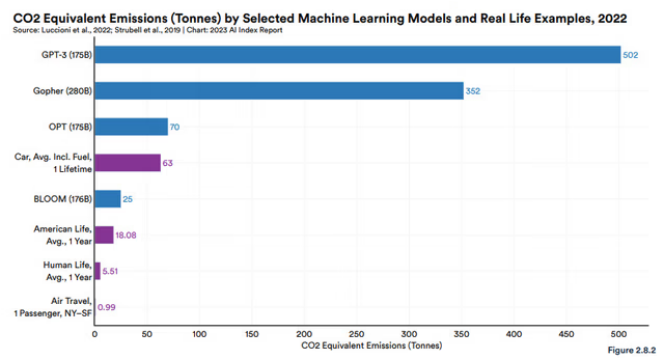
\includegraphics{figures/ai_co2.png}

}

\caption{\href{https://www.gizmodo.jp/2023/04/chatgpt-ai-openai-carbon-emissions-stanford-report.html}{LLMの環境負荷}}

\end{figure}

\hypertarget{ux4ebaux5de5ux77e5ux80fdux3068ux52b4ux50cd}{%
\subsubsection{人工知能と労働}\label{ux4ebaux5de5ux77e5ux80fdux3068ux52b4ux50cd}}

AIの発展によって雇用は減るのか?

\begin{itemize}
\tightlist
\item
  ラッダイト運動:産業革命\(\leadsto\)繊維産業の自動化\(\leadsto\)熟練工の抗議

  \begin{itemize}
  \tightlist
  \item
    自動化によって新しい雇用の創出&効率的な生産による生活水準の向上
  \item
    1755-1802年の労働者の実質賃金は半減、生活環境の悪化
  \end{itemize}
\end{itemize}

\begin{figure}[htpb]

{\centering 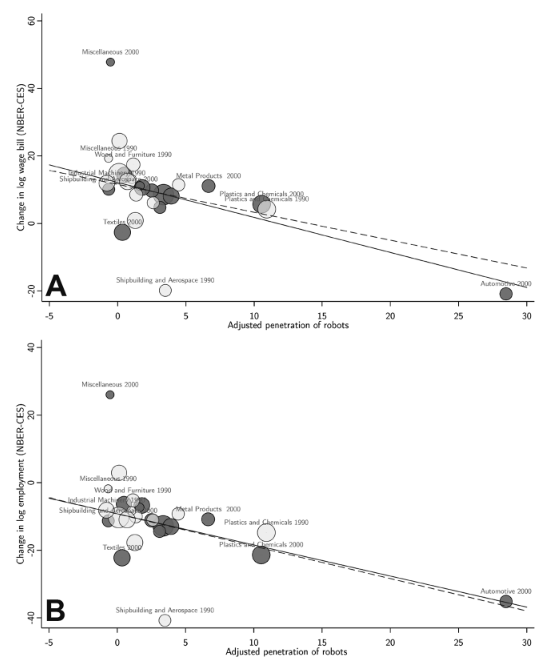
\includegraphics{figures/acemoglu.png}

}

\caption{\citet{acemoglu2020}}

\end{figure}

製造の自動化とは異なり、LLM(やその他の生成AI)によって代替される職業は?\citep{eloundou2023}

\hypertarget{ux6a5fux68b0ux5b66ux7fd2ux306eux5b9fux8df5}{%
\section{機械学習の実践}\label{ux6a5fux68b0ux5b66ux7fd2ux306eux5b9fux8df5}}

機械学習を初めとするデータ分析は様々な教材・資料がオンラインに無料で公開されている。

人工知能(の基盤にある機械学習)の多くは\textbf{Python}というプログラミング言語で実行

\begin{itemize}
\tightlist
\item
  制約付きではあるが\href{https://colab.research.google.com/}{Google
  Colaboratory}でオンラインで実行できる。
\item
  Python自体も無料なので、自分のPCにインストールして実行できる。

  \begin{itemize}
  \tightlist
  \item
    環境構築はちょっとめんどくさい
  \item
    jupyter notebookやvisual studio
    codeなどが人気のある\textbf{統合開発環境} (integrated development
    environment: IDE)
  \end{itemize}
\end{itemize}

パッケージをインストール・読み込む\(\leadsto\)様々な分析

\begin{itemize}
\tightlist
\item
  \href{https://pandas.pydata.org/}{pandas}:データの読み込み、処理
\item
  \href{https://matplotlib.org/}{matpoltlib},
  \href{https://seaborn.pydata.org/}{seaborn}:グラフの作成
\item
  \href{https://scikit-learn.org/stable/}{sicikit-learn}:(深層学習を除く)機械学習
\item
  \href{https://www.statsmodels.org/stable/}{statsmodels}:統計分析
\end{itemize}

深層学習のライブラリとして\href{https://www.tensorflow.org/}{TensorFlow}、\href{https://pytorch.org/}{PyTorch}、\href{https://keras.io/ja/}{keras}など

\begin{itemize}
\tightlist
\item
  \href{https://www.tensorflow.org/tutorials}{TensorFlow
  Coreのチュートリアル}や\href{https://www.tensorflow.org/hub/tutorials}{TensorFlow
  Hubのチュートリアル}ではGoogle Colaboratoryで試すことができる。
\item
  まずは学習済みモデルを利用
\end{itemize}

\href{https://www.kaggle.com/}{Kaggle}や\href{https://signate.jp/}{Signate}、\href{https://www.nishika.com/}{Nishika}などのデータ分析コンペ

\begin{itemize}
\tightlist
\item
  学生向けのイベントもあり
\item
  就職活動でアピールできる(かも)
\end{itemize}


  \bibliography{references.bib}


\end{document}
